%%=============================================================================
%% Results
%%=============================================================================

\chapter{\IfLanguageName{dutch}{Resultaten}{Results}}%
\label{ch:results}

The result section focuses on elaborating conducted experiments and acquired results, divided into the three main phases, localization, segmentation and recognition. After discussing the first results, additional labels and fine-tuning is performed. The final amount of labels and results are added at the end. In order to label, annotate videos and gain insights in the results a Vue3 web-app is created on a python flask API which reads and stores labels and video annotations from a MySQL database. Furthermore, the experiments are all performed using an Acer Nitro ANV15-51, running Ubuntu 24.04.2 LTS, using a 13th Gen Intel® Core™ i5-13420H × 12, with 16GB RAM and a NVIDIA GeForce RTX™ 4050 Laptop GPU 5898MiB.

\section{Jumper localization}

% TODO: add, this is relevant
% TODO: convex hull the 3 jumpers and train on yolo model.
As DD3 routines are the focus of this research, the idea was to predict the coordinates and position of a team as a single unit, instead of individuals. This idea was supported by the fact that there aren't any public jump rope datasets and it was expected to increase the speed of labeling. The AI generated image \ref{fig:sr2-performance-ai-generated} shows an example of a competition setting where two athletes are performing a routine. The goal here would be to crop out the jumpers.

% TODO : add crop around jupers

Below you can find a shortlist of experiments executed on localization.

\begin{itemize}
    \item random conv
    \item googlenet, mobilenet...
    \item Labeling individual jumpers \& pre-trained model yolo -> OK
\end{itemize}

\subsection{Random convolutional network}

% TODO : illustrative image of box coords?

Before discussing the different results, let's discuss how the location of skippers are marked. To mark the position of an object on an image, there are multiple possibilities.
For this project, the relative center point along the x-axis, y-axis, width and height of the box are stored. So regardless of the scale of the image, whether the image has size 1920 x 1080 pixels or 1080 x 720 pixels, the position of the box remains the same.
An example of a box would be [0.6, 0.5, 0.4, 0.4], all values between 0 and 1. IoU accuracy can then be performed.
... As explained in the literature (todo reference/add to literature)...
% TODO : shift IoU comparison to literature

(TODO: expand)
In order to get an idea, whether following models are able to learn, a random convolutional network is created.
... elaborate results % TODO

-> low accuracy, naive predictions.

To get a first idea whether it would start learning, so a transition can be made towards more advanced architectures.

\subsection{Dedicated architectures}

(TODO : expand)
Trained from scratch

GoogleNet, MobileNet... (on individual labels)

Display code \& mention unbalanced augmented, but still unbalanced dataset \& higher learning rate as compared below.

Conclusion:
Predicting full teams didn't work out which allowed for a transition to labeling and predicting individuals athletes. Below you find more information about those experiments.

\subsection{YOLO}

Experiment 3, pre-trained models \& individual boxes.

The third experiment incorporates a double upgrade. The first upgrade involves annotating individual athletes on images instead of one big box around all jumpers. This method allows to annotate other routines such as single rope, chinese wheel or double dutch 4. The second upgrade is trying a pre-trained object detection model.

Ultralytics \autocite{Khanam2024} provides an easy-to-use pre-trained implementation for predicting people and objects in images which can be fine-tuned for specific use cases. Fine-tuning was needed as spectators, also humans, were also included in the predictions.

Using these predictions, a crop around the three jumpers can be created using the predicted jumper boxes from the fine-tuned YOLO model, after using the pre-trained weights on the COCO dataset \autocite{Lin2014}. In order to improve the crops some steps were required. Details are discussed below.

\subsubsection{Crop stability}

\begin{figure}
    \centering
    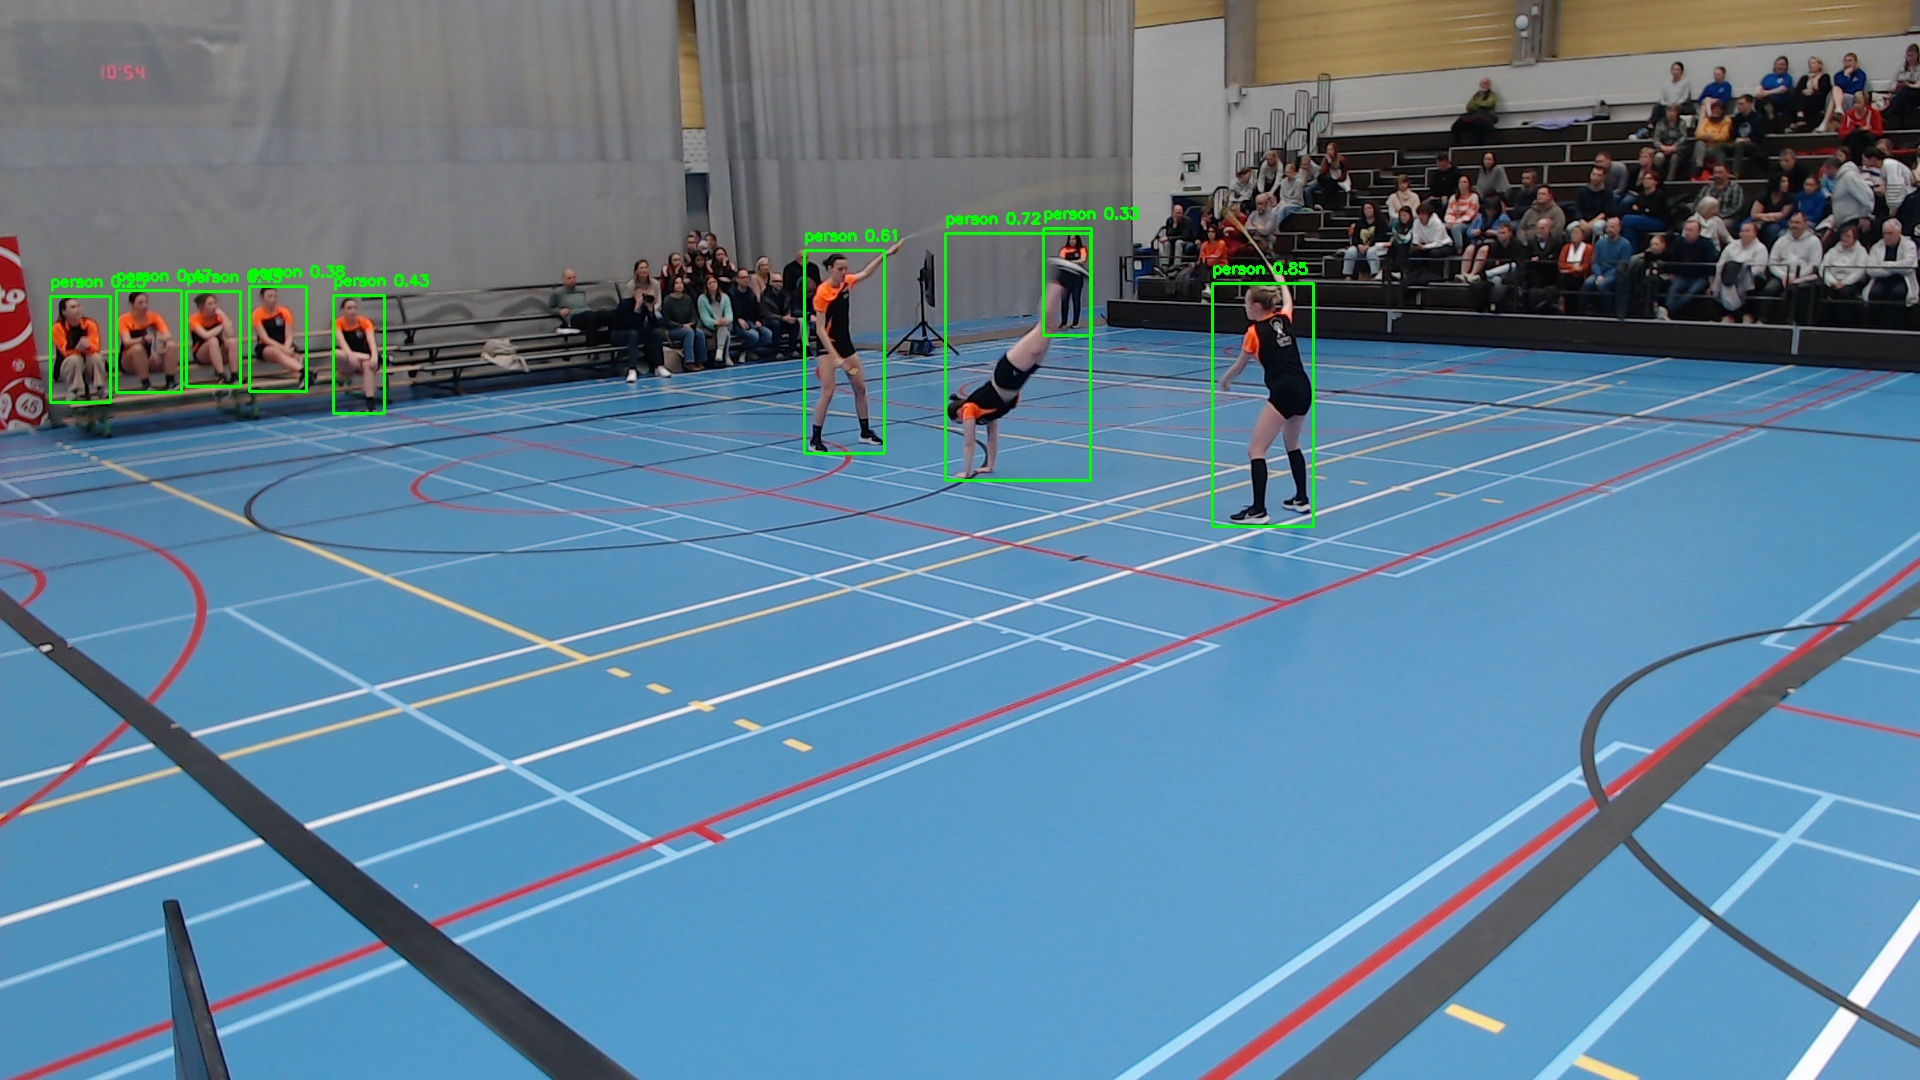
\includegraphics[width=0.95\linewidth]{img/1267_292_boxes}
    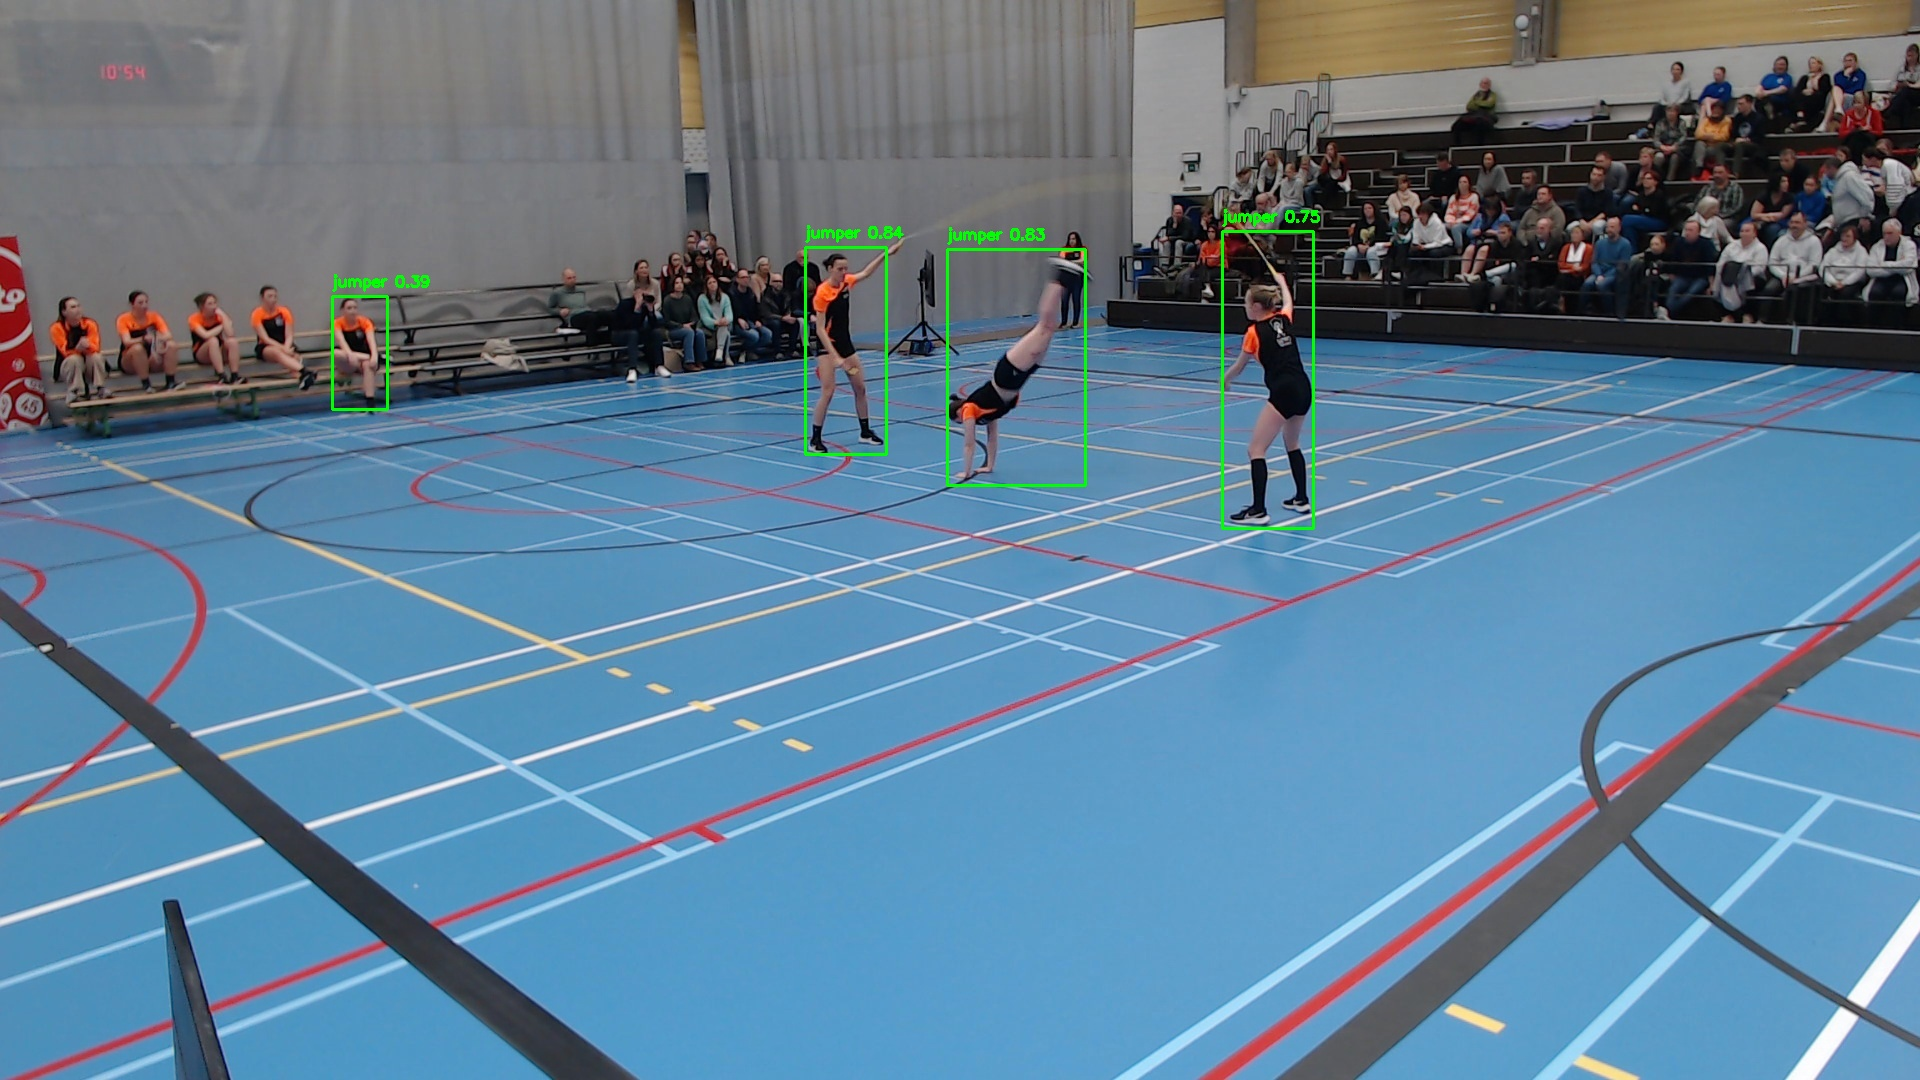
\includegraphics[width=0.95\linewidth]{img/1267_292_boxes_reduced_spectators}
    \caption[raw vs fine-tuned YOLOv11 nano model predictions]{Raw predictions of the unrefined YOLOv11 nano model compared to the fine-tuned model which reduces predictions of spectators.}
    \label{fig:raw-vs-fine-tuned-boxes}
\end{figure}

\begin{figure}
    \centering
%%    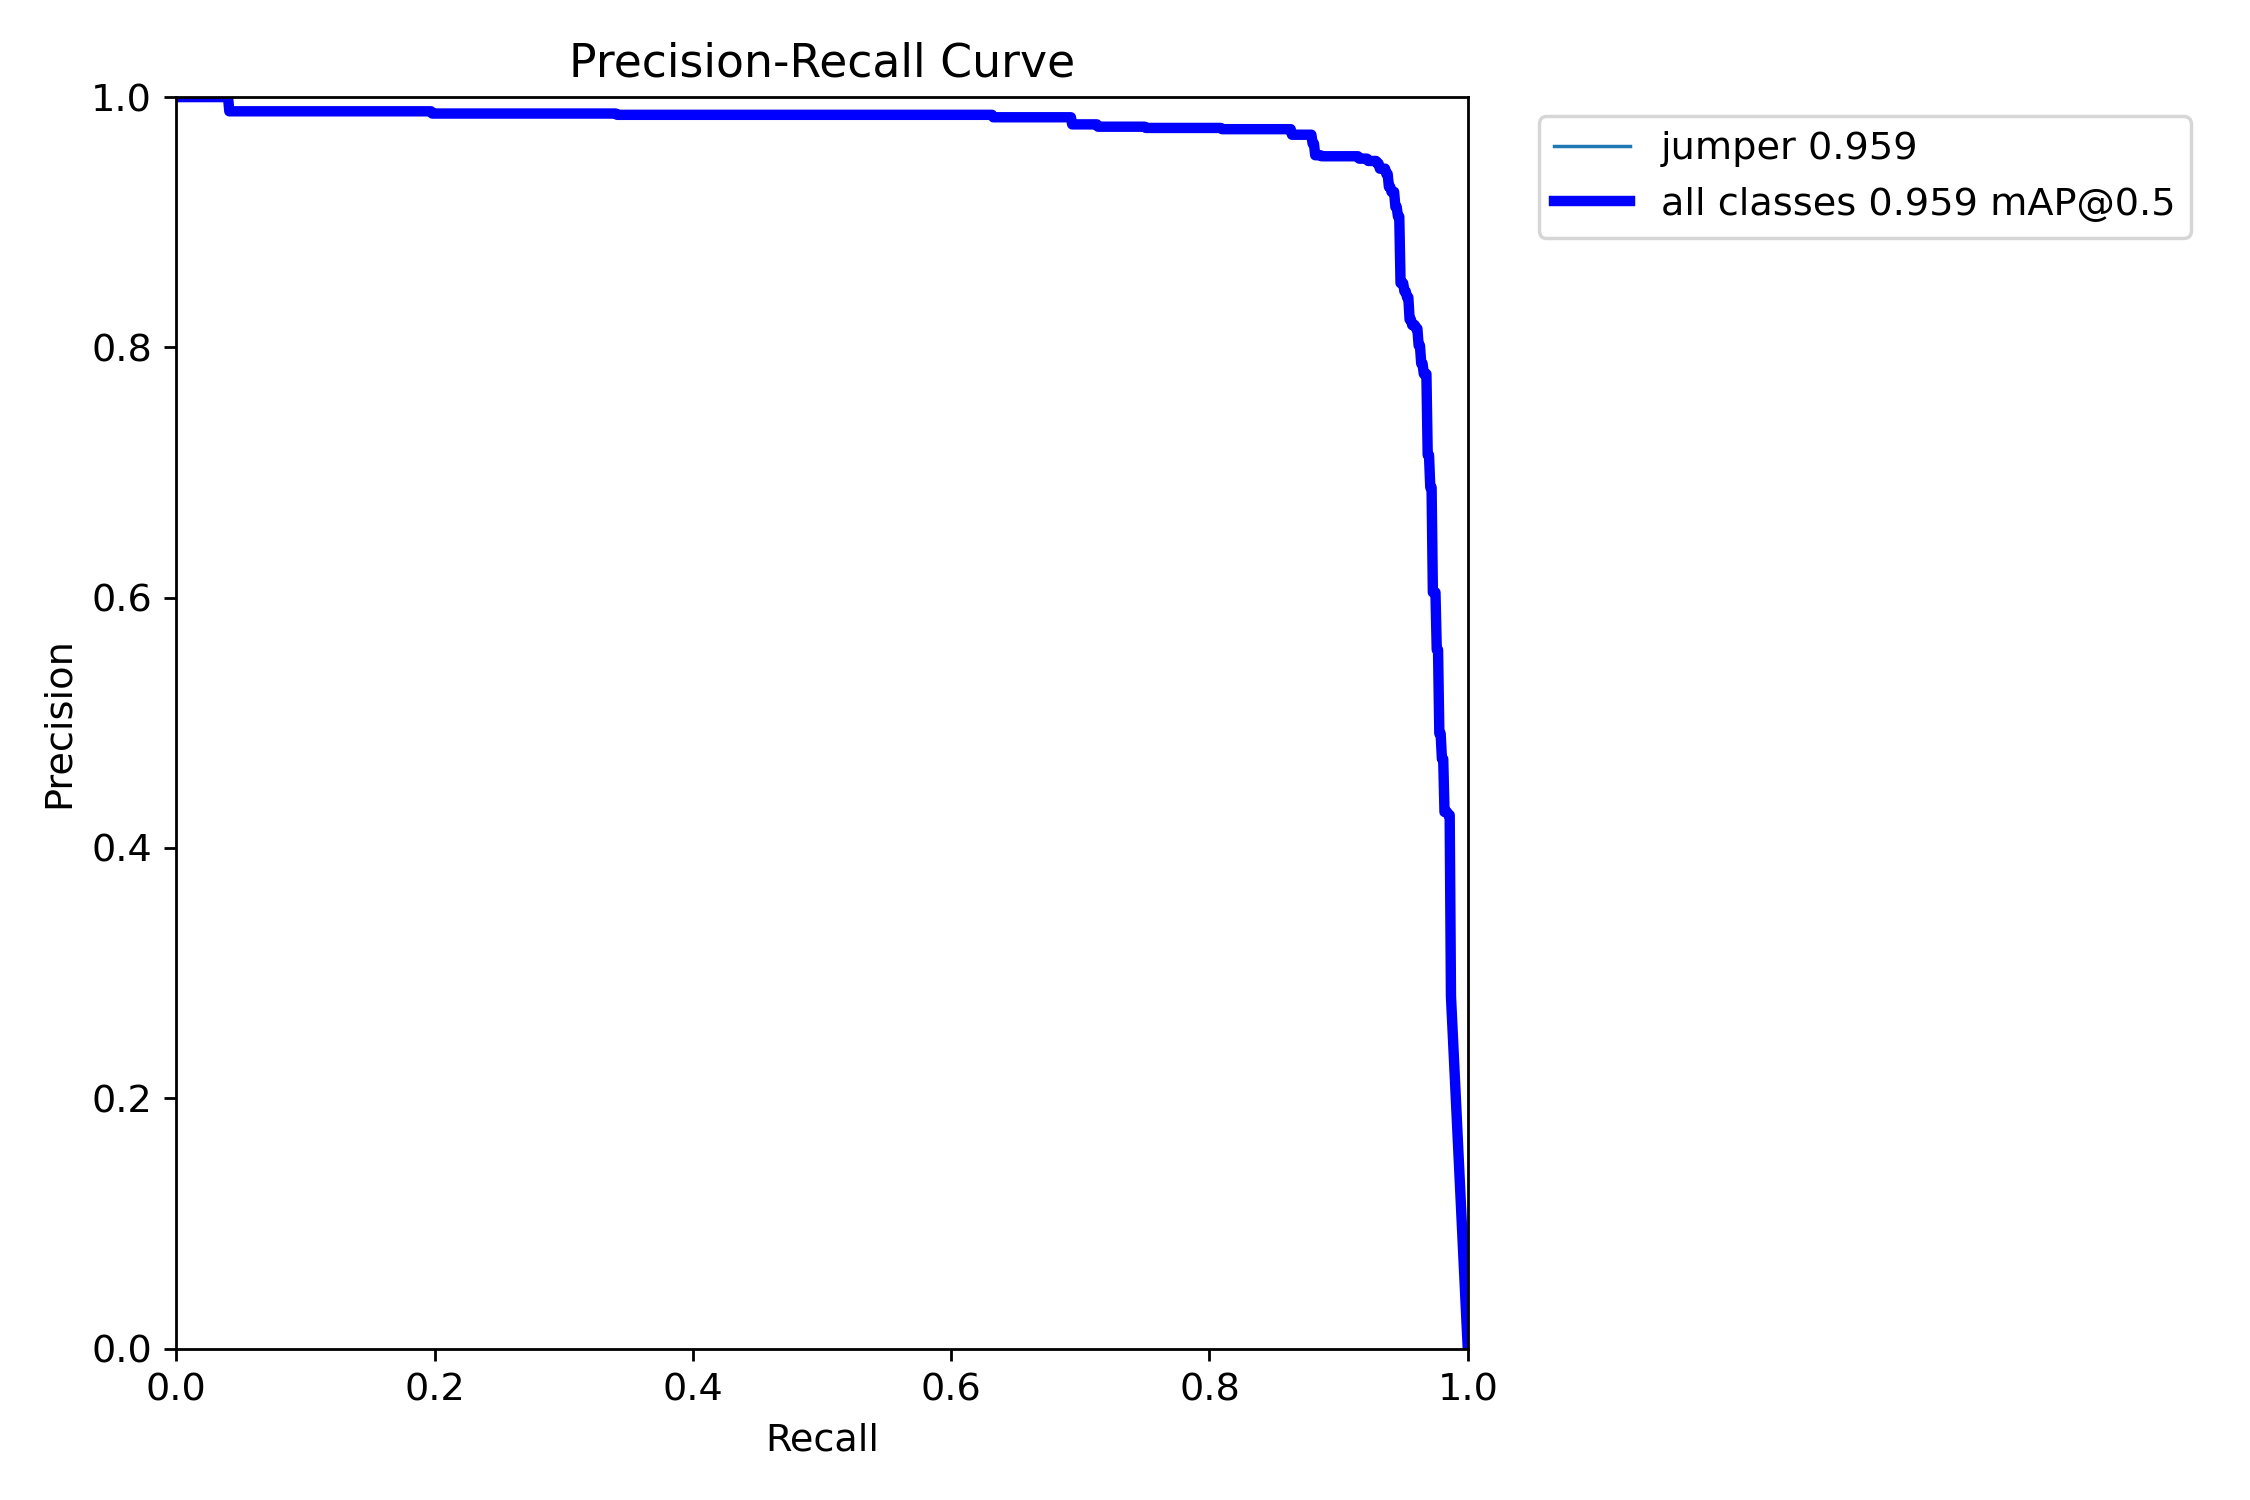
\includegraphics[width=0.35\linewidth]{img/PR_curve}
    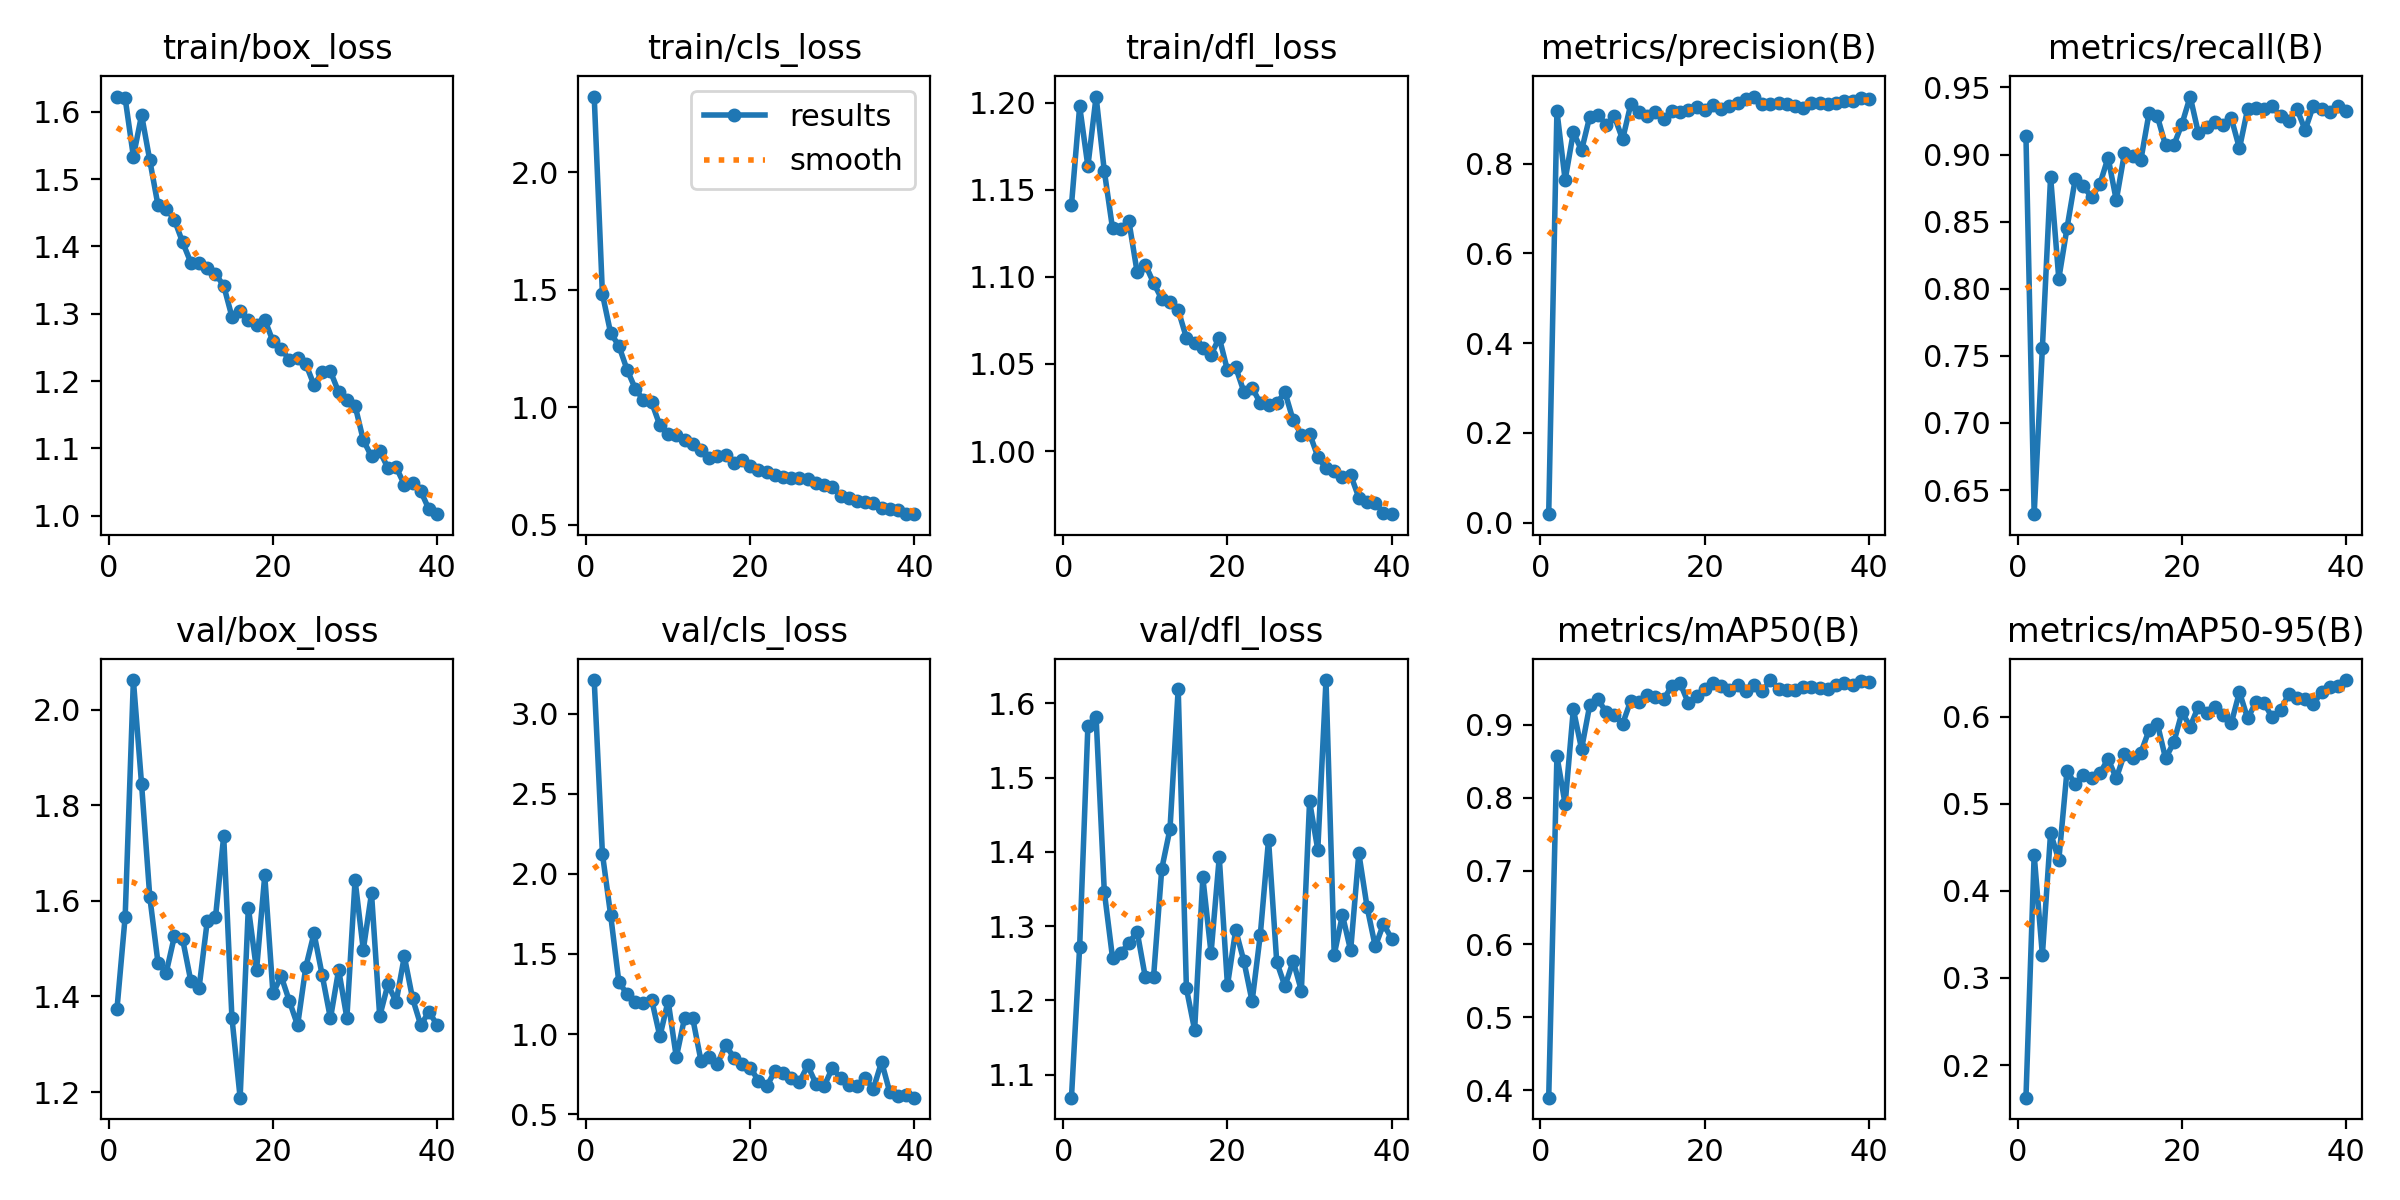
\includegraphics[width=0.95\linewidth]{img/results}
    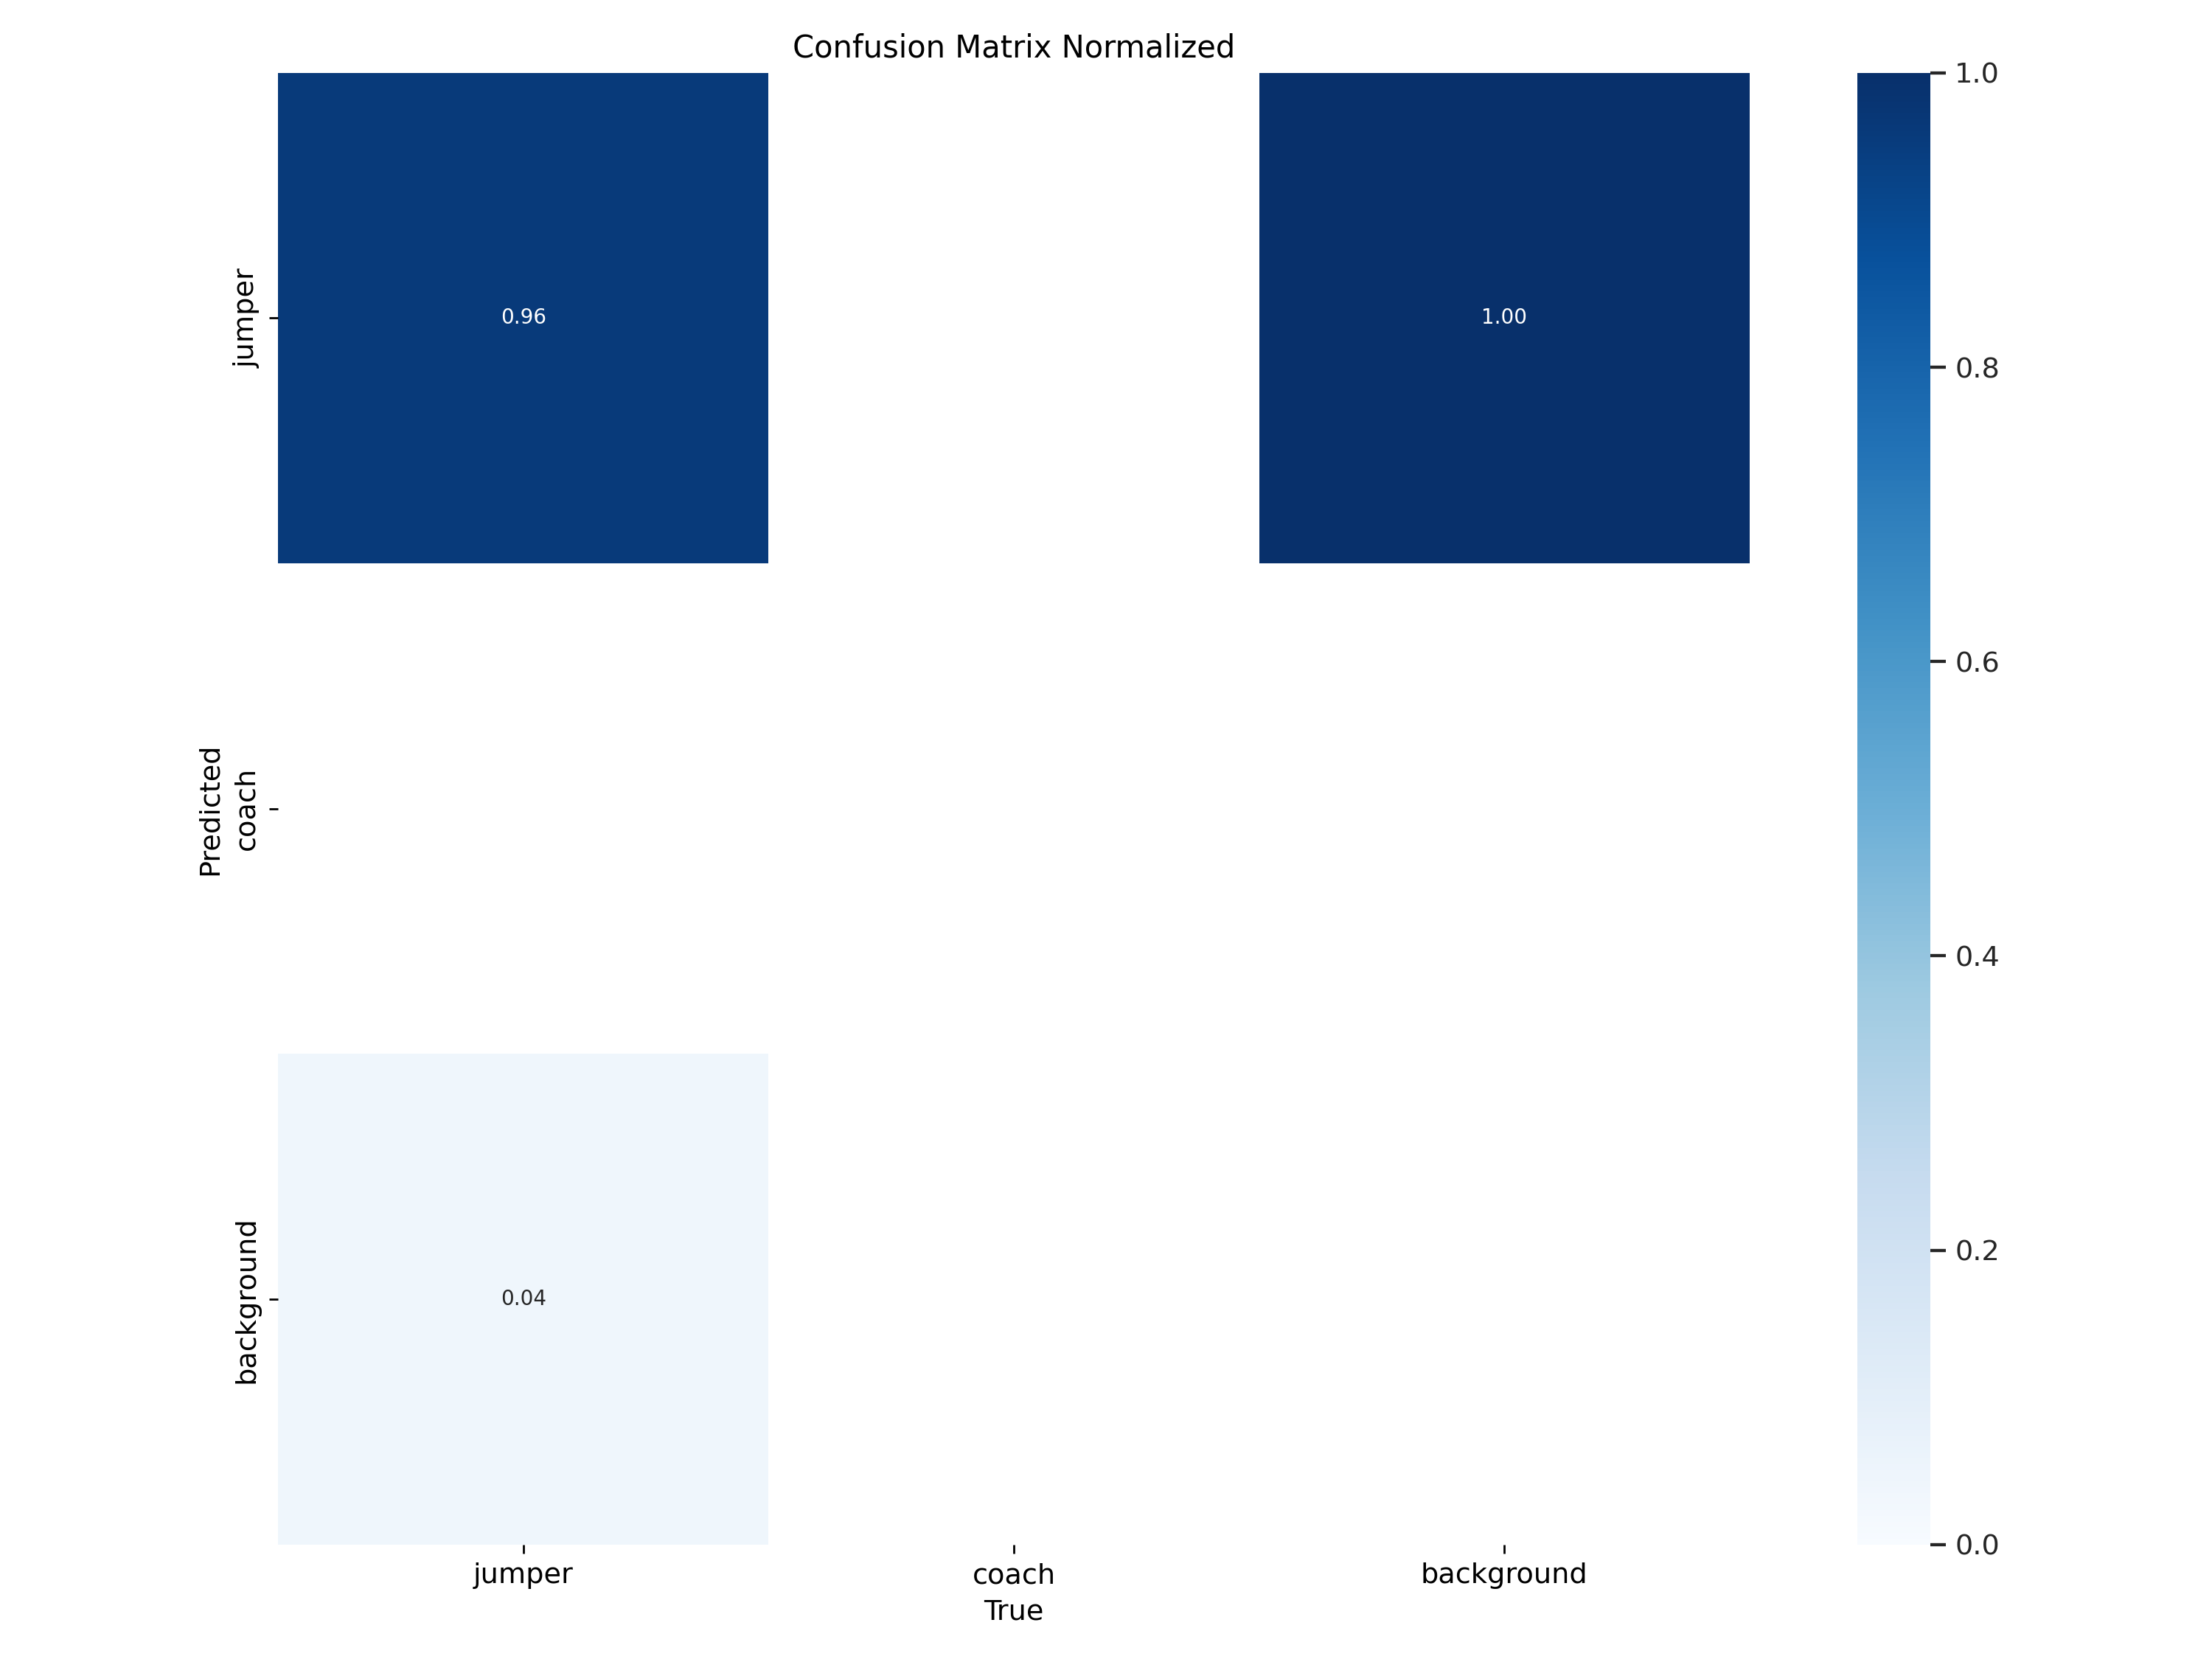
\includegraphics[width=0.85\linewidth]{img/confusion_matrix_normalized}
    \caption[metrics after fine-tuning YOLOv11]{Metrics after fine-tuning YOLOv11 on the validation set of 161 images, mAP50 of 0.953 \& mAP50-95 of 0.63, annotation of coaches was an idea.}
    \label{fig:localization-results}
\end{figure}

\begin{figure}
    \centering
    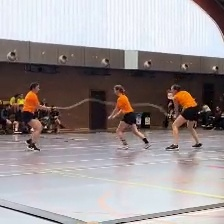
\includegraphics[width=0.45\linewidth]{img/1315_2935}
    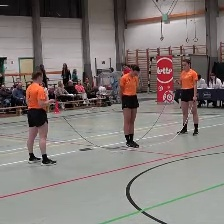
\includegraphics[width=0.45\linewidth]{img/2297_134}
    \caption[Valid crops of a DD3 routine on competition.]{Valid crops of a DD3 routine on competition. (224x244 pixels)}
    \label{fig:dd3-crop}
\end{figure}

\begin{figure}
    \centering
    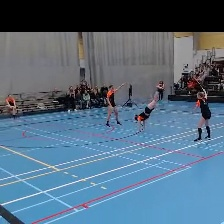
\includegraphics[width=0.45\linewidth]{img/1267_292_cropped}
    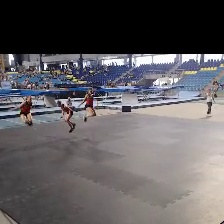
\includegraphics[width=0.45\linewidth]{img/1405_1061_cropped}
    \caption[dd3-crop-error]{Two crops including a spectator alongside the athletes.}
    \label{fig:dd3-crop-error}
\end{figure}

Annotating only athletes on 732 images \& fine-tuning the pre-trained nano yolo model, the first predictions of spectators are reduced considerately.
This way crops can be created by taking the minimum and maximum \(x\) \& \(y\)-coordinates. Reviewing cropped videos show indicate occasional frames predicting spectators, coaches or judges and moments of instability, as if you are watching camera footage of an earthquake.

In order to avoid a sudden zoom out, because of spectators, an IoU comparison of the previous predicted box with the new box is made. If the IoU value is larger than the average IoU of the last \(N\) seconds, powered to the fourth, than crop coordinates will be updated. Using this IoU comparison, reduces video crops including spectators, maintaining the earthquake effect.


To reduce shakiness and maintain a nice to watch cropped video, box-coordinates are smoothed out adapting box predictions of previous frames with the current one. This way, drastic changes in a predicted location, e.g. model error, arm or field movements aren't that drastic. Adaptation is done by incorporating two smooth values, indicating how much weight you give to the smoothed prediction of the previous frame. \footnote{Smoothed values are obtained by playing around with values, choosing those leading to the best, subjective, smoothed review}

$$ smth = smootval = 0.86  \quad \& \quad smths = smootval\_shrink = 0.94 $$

Which makes the new coordinates:

\begin{math}
   smooted_{x1_{min}} =
   \begin{cases}
       smooted_{x1_{min}} & \text{if} \quad iou < iou_{threshold} \\
       smth * smooted_{x1_{min}} + (1-smth) * x1_{min} & \text{else if} \quad x1_{min} < smooted_{x1_{min}} \\
       smths^ * smooted_{x1_{min}} + (1-smths) * x1_{min} & \text{otherwise}
   \end{cases}
\end{math}

The same is done for \( y1_{min}, x2_{max}, y2_{max} \).

Utilizing these steps allows for videos where a team is always on display (\ref{fig:dd3-crop}), with some videos still predicting spectators (\ref{fig:dd3-crop-error}) and a newly introduced problem, namely skippers running out of view.

% TODO : add movement corrector

\begin{figure}
    \centering
    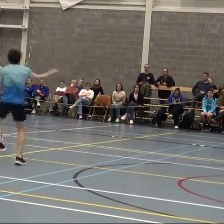
\includegraphics[width=0.45\linewidth]{img/1241_1093_cropped}
    \caption[dd3-crop-error]{Athletes running out of view.}
    \label{fig:dd3-crop-error-out-of-view}
\end{figure}

One way to solve jumpers running out of view, is by adding a default movement corrector, like the smooth value, which follows the new coordinates every frame. The movement corrector is based on the \(iou\)-value powered to the \(1/8\). It makes the crop following predictions by default, when IoU is getting low.


\begin{math}
    SQRT = 8 \\
    movementCorrector = iou^{1/SQRT} \\
    smooted_{x1_{min}} = smooted_{x1_{min}} * movementCorrector + (1 - movementCorrector) * {x1_{min}}
\end{math}



A possible improvement could be matching individual boxes with the new predictions, eliminating the spectator. Which raises concerns about jumpers entering the competition field. There are no earlier predicted boxes to match.
The total algorithm isn't perfect yet, but the results indicate sufficient valid video crops to use and experiment on segmentation and recognition.

\begin{listing}
    \begin{minted}{python}
        print('TODO : cleanup code')
    \end{minted}
    \caption[Example codefragment]{Example of adding cropping code.}
    \label{code:localization}
\end{listing}

Full code is visible in code snippet \ref{code:localization}. The results are broken down in table \ref{tbl:crop-results}. In this table you can see that about 15\% of the videos aren't localized properly, some of them only have minor disturbs. This results in enough videos available to try and recognize skills.

% TODO: pairwise distances?

\begin{table}[h!]
    \begin{tabular}{|l|l|l|}
        \hline
        \textbf{videoId} & \textbf{seconds} & \textbf{reason} \\
        \hline
        \dots & \cellcolor{green!25} \dots & (other videos) \\ \hline
        1435 &	\cellcolor{green!25} 0 &	 \\ \hline
        1445 &	\cellcolor{green!25} 0 &	 \\ \hline
        2285 &	\cellcolor{green!25} 0 &	 \\ \hline
        2295 &	\cellcolor{green!25} 0 &	 \\ \hline
        2305 &	\cellcolor{green!25} 0 &	 \\ \hline
        2315 &	\cellcolor{green!25} 0 &	 \\ \hline
        995  &	\cellcolor{yellow!25} 5 &	Schocks \& turner out-of-view \\ \hline
        1275 &	\cellcolor{yellow!25} 1 &	aerial half \\ \hline
        1405 &	\cellcolor{orange!25} 30 &	spectator \\ \hline
        651  &	\cellcolor{yellow!25} 1    &	turner out of view \\ \hline
        664  &	\cellcolor{yellow!25} 1.5  &	turner out of view \\ \hline
        1202 &	\cellcolor{yellow!25} 5    &	turner out of view, recording itself \\ \hline
        1178 &	\cellcolor{yellow!25} 2    &	turner out of view \\ \hline
        1238 &	\cellcolor{yellow!25} 2    &	spectator before start routine \\ \hline
        1244 &	\cellcolor{yellow!25} 0    &	stopped following, remained in view \\ \hline
        1257 &	\cellcolor{yellow!25} 0    &	stopped following, remained in view \\ \hline
        1275 &	\cellcolor{yellow!25} 1.5  &	half out of view \\ \hline
        1339 &	\cellcolor{yellow!25} 8    &  spectator \\ \hline
        1444 &	\cellcolor{yellow!25} 1.5  &	half out of view \\ \hline
        2282 &	\cellcolor{yellow!25} 1    &	1 turner out of view, actual 3 sec no follow \\ \hline
        2317 &	\cellcolor{yellow!25} 2    &	minor shocks \\ \hline
        663  &	\cellcolor{orange!25} 25   &	Out-of-view \& shocks \\ \hline
        1241 &	\cellcolor{orange!25} 8    &	Out-of-view \\ \hline
        1267 &	\cellcolor{orange!25} 46   &	spectator \\ \hline
        1271 &	\cellcolor{orange!25} 24   &	Out-of-view \\ \hline
        1273 &	\cellcolor{orange!25} 8    &	Out-of-view \\ \hline
        1326 &	\cellcolor{orange!25} 6.5  &	spectator \\ \hline
        \(avg\) &	1.33 &	(seconds / 1m15) \\ \hline
        \(avg_{if}\) &	8.55 &	(seconds / 1m15) \\ \hline
        Nr of videos not ok &	21	& 15.6\% \\ \hline
        Total checked videos &	135	& (includes train videos) \\ \hline
    \end{tabular}
    \caption[Manually checked crop results]{Crop results manually checked on the amount of seconds where a crop is disturbing. The reason why it is disturbing is added in the reason column, this could be athletes out of view, unstable/earthquake like predictions... \\
    Yellow indicated videos are not disturbing for recognition, even though the crops aren't perfect. Orange videos require more attention and shouldn't be used for recognition. \\
    The \(avg_{if}\) indicates the average time in case a video has crops which aren't good.}
    \label{tbl:crop-results}
\end{table}


\subsection{Full video crops - automated testing (Work in Progress - WIP)}

As manual checking videos can be time consuming, automated tests are in progress of creation in order to check whether crop strategies work or not.
Utilizing the 7k legacy labels of full team boxes, video crops are calculated for each strategy.
Both train and validation will be added separately in the results as there are less trainings videos labeled with individual boxes (129) than there are full box annotations on the trainings videos (325).
The code for localizing has been cleaned as well. % (TODO add)














\section{Action segmentation}

Experiments on action segmentation have waited on skill recognition (section \ref{results:recognition}), this is why the experiments with action segmentation use the same models as the skill recognition, adapting only the top layers of the models.

To annotate which moments are interesting split points, the start and end frame of a skill receive value 1, while other frames remain 0.
As the start and end frame of a skill are rather subjective, frames around a split point also range somewhere between 0 and 1. These values are calculated using the function \ref{code:calculate-splitpoint-values} which is called on in the data generator demonstrated in code \ref{code:call-splitpoint-calculation}.
Each frame than has a value from zero to one. An example of consecutive splitpointvalues could be:

\([0, 0, 0.1, 0.31, 0.55, 0.86, 1, 0.86, 0.55, 0.31, 0.1, 0]\)


\subsection{Video Vision Transformer \& Self-attention ConvLSTM}
\label{subsec:video-models-from-scratch}

The first and second experiment for segmention use code implementations of the Video Vision Transformer as developed in \textcite{Arnab2021} (ViViT - \ref{code:get_model_ViViT}) and the Self-Attention ConvLSTM from \textcite{Lin_2020} (SA-ConvLSTM - (TODO)).
To resolve bugs and dimensionality issues, Large Language models are used (\autocite{OpenAI_ChatGPT_2025} and \autocite{Deepseek_2025}).
These models were then trained on 7.8k batches of 16 consecutive frames, which originate from 44 trainings videos for about 48 minutes of training data, having framerates between 25 and 60 \footnote{Most labeled videos have a framerate of 25, 30 or 50 frames per second} images per second.
Both models showed the same results, averaging out predictions slightly above 0 for all frames, stagnating on MSE losses of around 0.09 and 0.10. This was about the average when always predicting 0. (Exact values are lost due to the switch to pytorch and bugs, will/could be re-added later.)

\subsection{Pre-trained MViT}

In order to get better results on the little labeled available data, (44 videos for training, 7 validation videos), looking for a pre-trained model really helped a lot.
PyTorch provides a \href{https://pytorch.org/vision/main/models.html}{list} of pre-build and pre-trained models such as \href{https://pytorch.org/vision/main/models/video_mvit.html}{mvit-v1-b}.
Fine-tuning this model lowered the MSE to 0.065 with peaks overlapping splitpoints as demonstrated and elaborated in figure \ref{fig:segmentation-plot}.

To get al sections, all peaks in its neighborhood (\(windowsize = fps / 3\)) having a splitpoint value more than 0.4 become the start and end frame of a skill section, which will be used to recognize which skill is displayed. The code filtering segments out of raw-predicted splitpoint values is \ref{code:predictions-to-splitpoints}, filtering peaks (fig  \ref{fig:segmentation-plot}) in a list of start and end frames. An example could be \([...2280, 2320, 2355, 2382...]\), as splitpoints.


\begin{figure}
    \centering
    \includegraphics[width=0.45\linewidth]{img/segmentplot_2285_frameStart_2250_with_250_points}
    \includegraphics[width=0.45\linewidth]{img/segmentplot_2285_frameStart_2500_with_250_points}
    \includegraphics[width=0.45\linewidth]{img/segmentplot_2285_frameStart_2750_with_250_points}
    \includegraphics[width=0.45\linewidth]{img/segmentplot_2285_frameStart_3000_with_250_points}
    \caption[Segmentation plot]{Segmentation plot comparing predictions with the splitpoint values indicating a match of interesting splitpoint. Visible errors are: \\
        at frame 2459, a relatively lower jump out of the rope with a snapper. \\
        at frames 2700 until 2900 indicating a transition which is labeled in one segment, but the athletes are rather bouncy on their feet, letting the model think those are splitpoints. \\
        a handspring occurs from frame 3140 until 3192, but the model indicates to much during the skill, while it doesn't indicate the moment right after the handspring.
    }
    \label{fig:segmentation-plot}
\end{figure}

(Ideas for additional metrics such as avg distance between nearest peak and splitpoint, IoU like overlap with nearest peaks will follow later \& further research on segmentation will follow in another submit.)

These predicted segments are the first usable split moments to use for splitting unseen videos recognizing or speeding up further labeling.

% TODO : transition

\section{Skill recognition}
\label{results:recognition}

\begin{figure}
    \centering
    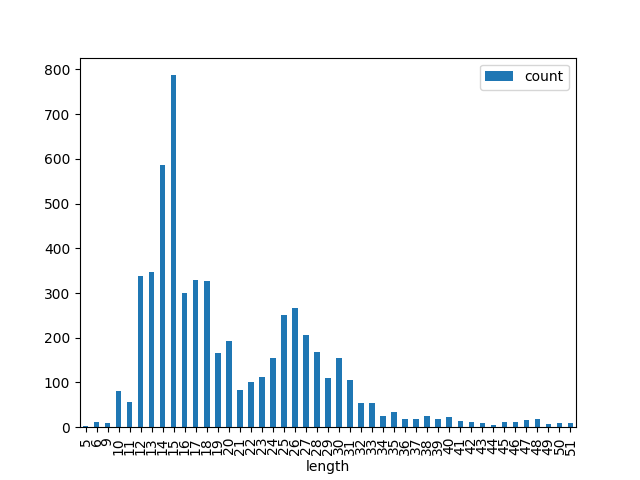
\includegraphics[width=0.95\linewidth]{img/skilllengths}
    \caption[frame counts of skill lengths]{Distribution of skill length (in frames), visually limited to 50 frames per skill. Skill lengths differ depending on the frame rate of the video. Most videos have a framerate of 25, 30 or 50. Annotated sections longer than 50 frames are mostly transitions, mistake recoveries, gymnastic typed skills or powerskills with more than one rotation.}
    \label{fig:skilllengths-counts}
\end{figure}


Having small little sections of potential skills (normal jumps, and mistake recoveries included) allows to predict what actions are actually in this section.
As the segments provided by the segmentation model have a varying frame count, and the length of skills in general can differ, they need to be transformed in equal sized frames.
Depending on the frame rate, most skills have a frame rate between 12 and 18 frames per skill, see figure \ref{fig:skilllengths-counts} for a distribution. In order to transform skills into equally sized sections, frames are skipped or duplicated depending on the length of the skill.
The selected frames are calculated in code snippet \ref{code:skill-frame-selection}.


\begin{listing}
    \begin{minted}{python}
        timesteps = 16
        slot = skill_length_over_timesteps = skill_length / timesteps
        frames [frames_skill[round(i * slot)] for i in range(timesteps)]
    \end{minted}
    \caption[Code for frame selection skills]{Code for frame selection of skills}
    \label{code:skill-frame-selection}
\end{listing}



\subsection{Video Vision Transformer \& Self-attention ConvLSTM}

Using about 5k skills, 4550 to train and 669 to validate, the same video models as described in the segmentation phase \ref{subsec:video-models-from-scratch} can be trained the skill properties defined in \ref{subsec:skillcomplexiteit}.
During the annotation of videos, it is noticed how screwed the skill-data is. Other action properties like turners, hands, type or faults are equally skewed. See table \ref{tab:skill_distribution_full_with_nulls} for a breakdown of skill occurrences.

Both the ViViT and the SA-ConvLSTM were plateauing on the most appearing value, always predicting normal jumps, normally turned, without a mistake etc.
Even up-sampling less occurring combination didn't help. The models stagnated on validation losses of 5.9 and 6.5. See figure \ref{fig:skill-upsampling-distribution} to see how many times a skill appears in a training round, depending on its uniqueness.

\begin{figure}
    \centering
    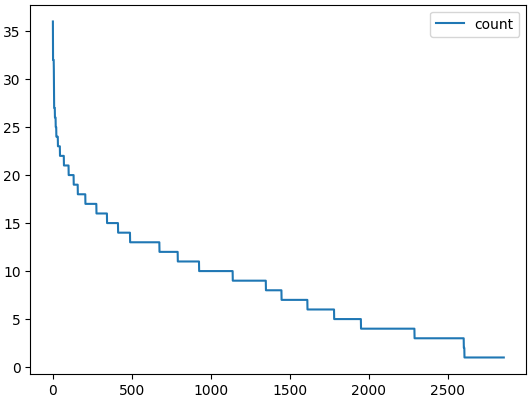
\includegraphics[width=0.7\linewidth]{img/skill-upsampling-distribution}
    \caption[upsampling distribution of skills]{Occurance of each labeled skill (e.g. videoId 123, frameStart 480, frameEnd 504, Double Dutch, 1 rotation, split, EB, crouger...) in the upsampeled dataset. Values get duplicated based on the uniqueness of each property. E.g. because it is an EB and a split, it will be duplicated four times, but no/less duplication because Double Dutch and 1 rotation is more common.}
    \label{fig:skill-upsampling-distribution}
\end{figure}

In order to reach better results, the search for a pre-trained model leads us to the following experiment, namely the usage of PyTorch implementation of the Multiscale Video Vision Transformer.

\subsection{Multiscale Video Vision Transformer - MViT}


\begin{figure}
    \centering
    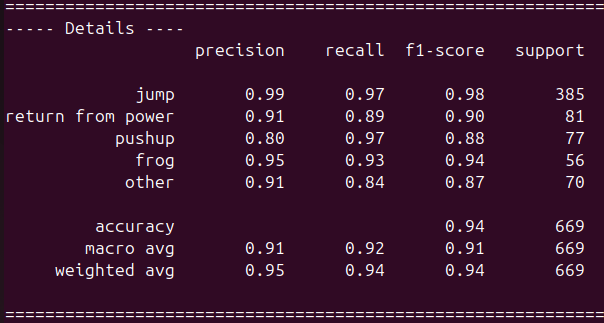
\includegraphics[width=0.7\linewidth]{img/mvit-5-classes}
    \caption[Classification report on only 5 skill classes]{Classification report on the 5 classes jumps, pushups, return from powers, frogs or other skills after training mvit on an equally distributed, max 442 samples per skill as seen in table \ref{tab:skill_distribution_grouped_final}.}
    \label{fig:mvit-5-classes}
\end{figure}


\href{https://pytorch.org/vision/main/models/video_mvit.html}{PyTorch's Video MViT} is an implementation based on the Multiscale Vision Transformer created by \textcite{Fan2021} and possibly pre-trained on the kinetics dataset.
The first experiment using this model used a perfectly balanced dataset for skills only, namely taking a random subset of maximum of 442 samples on each of the 5 classes seen in table \ref{tab:skill_distribution_grouped_final}.
The first results showed accuracies of 87\% to 98\% (see fig. \ref{fig:mvit-5-classes}) even some turner skills getting predicted correctly.

Re-enabling all skill classes and all other properties results in a total validation loss of 1.3835, as compared to 5.9 or 6.5 earlier.
For skills only, the weighted f1-accuracy is 93\%, while macro f1-accuracy is 40\%.
The macro accuracy gives a better indication as accuracies on all defined classes, e.g. pushup, jump, swift, are taken into account equally. In this experiment, the less appearing skills lower the score of the macro accuracy, as they do not appear as often.

Like the previous subsection, these results are trained on the skilldistribution displayed in table \ref{tab:skill_distribution_full_with_nulls}).
A breakdown of all classification reports can be found in tables \ref{tbl:mvit-class-report-type} -> \ref{tbl:mvit-class-report-fault}. You may notice that the predictions for bodyRotations, sloppy, hard2see \& faults have yet to start learning.

\begin{table}[h!]
    \centering
    \begin{tabular}{|r|r|l|r|r|}
        \hline
        \textbf{Train \%} & \textbf{Train Count} & \textbf{Skill} & \textbf{Val Count} & \textbf{Val \%} \\
        \hline
        50.6687 & 2273 & jump & 379 & 56.6517 \\
        14.0660 & 631 & pushup & 77 & 11.5097 \\
        13.0629 & 586 & return from power & 84 & 12.5561 \\
        9.8529 & 442 & frog & 59 & 8.8191 \\
        3.2100 & 144 & crab & 9 & 1.3453 \\
        2.0062 & 90 & split & 12 & 1.7937 \\
        1.1146 & 50 & flip & 5 & 0.7474 \\
        0.9140 & 41 & rondat & 5 & 0.7474 \\
        0.8917 & 40 & rad & 3 & 0.4484 \\
        0.8025 & 36 & suicide & 8 & 1.1958 \\
        0.7356 & 33 & handspring & 5 & 0.7474 \\
        0.6910 & 31 & rol2kip & 7 & 1.0463 \\
        0.4458 & 20 & kip & 6 & 0.8969 \\
        0.3567 & 16 & speed & NULL & NULL \\
        0.3121 & 14 & kopkip & 1 & 0.1495 \\
        0.2675 & 12 & roll & 3 & 0.4484 \\
        0.1783 & 8 & stut & 2 & 0.2990 \\
        0.1337 & 6 & swift & NULL & NULL \\
        0.1337 & 6 & UNKOWN & 1 & 0.1495 \\
        0.0669 & 3 & leapfrog & NULL & NULL \\
        0.0446 & 2 & footwork-kick & NULL & NULL \\
        0.0223 & 1 & mountainclimber & NULL & NULL \\
        0.0223 & 1 & footwork-open & 1 & 0.1495 \\
        \hline
    \end{tabular}
    \caption[Skill distribution skill]{Skill distribution with training and validation counts and percentages. Null values indicate absence of skill occurrence in the validation data.}
    \label{tab:skill_distribution_full_with_nulls}
\end{table}


\begin{table}[h!]
    \centering
    \begin{tabular}{|l|r|r|r|r|}
        \hline
        \textbf{Skill} & \textbf{Train Count} & \textbf{Train \%} & \textbf{Val Count} & \textbf{Val \%} \\
        \hline
        jump & 2273 & 50.6687 & 379 & 56.6517 \\
        pushup & 631 & 14.0660 & 77 & 11.5097 \\
        return from power & 586 & 13.0629 & 84 & 12.5561 \\
        frog & 442 & 9.8529 & 59 & 8.8191 \\
        other & 526 & 11.7253 & 68 & 10.1645 \\
        \hline
    \end{tabular}
    \caption[Skill distribution skills limited classes]{Train and validation skill distribution with low-frequency skills grouped as "other"}
    \label{tab:skill_distribution_grouped_final}
\end{table}


\section{Model verification - act as a judge}

Comming soon... (Mapping predicted skills, turners, rotations... to its perspective level which will be compared with the score assigned by judges on competition.)

\begin{table}[h!]
    \begin{tabular}{|l|r|r|r|r|}
        \hline          & precision & recall & f1-score & support \\
        \hline
        Double Dutch    &   0.97    &   0.98    &   0.97    &  525 \\
        Single Dutch    &   1.00    &   0.25    &   0.40    &  4   \\
        Irish Dutch     &   0.00    &   0.00    &   0.00    &  0   \\
        Chinese Wheel   &   0.92    &   0.97    &   0.94    &  86  \\
        Transition      &   0.72    &   0.88    &   0.79    &  24  \\
        Snapperlike     &   0.90    &   0.63    &   0.75    &  30  \\
        \hline
        accuracy        &           &           &   0.95    &  669 \\
        macro avg       &   0.75    &   0.62    &   0.64    &  669 \\
        weighted avg    &   0.95    &   0.95    &   0.95    &  669 \\ \hline
    \end{tabular}
    \caption[Type distribution]{mvit-class-report-type}
    \label{tbl:mvit-class-report-type}
\end{table}

\begin{table}[h!]
    \begin{tabular}{|l|r|r|r|r|}
        \hline
          &  precision &   recall & f1-score &  support \\ \hline
        0 &       0.00 &     0.00 &     0.00 &       26 \\
        1 &       0.91 &     0.95 &     0.93 &      544 \\
        2 &       0.59 &     0.67 &     0.63 &       70 \\
        3 &       0.39 &     0.44 &     0.41 &       16 \\
        4 &       0.50 &     0.10 &     0.17 &       10 \\
        5 &       0.00 &     0.00 &     0.00 &        2 \\
        8 &       0.00 &     0.00 &     0.00 &        1 \\
        \hline
        accuracy &            &          &     0.86 &      669 \\
        macro avg &       0.34 &     0.31 &     0.31 &      669 \\
        weighted avg &       0.82 &     0.86 &     0.83 &      669 \\ \hline
    \end{tabular}
    \caption[Rotation distribution]{mvit-class-report-rotations}
    \label{tbl:mvit-class-report-rotations}
\end{table}

\begin{table}[h!]
    \begin{tabular}{|l|r|r|r|r|}
                \hline & precision &   recall & f1-score &  support \\ \hline
               normal &      0.93 &     0.98 &     0.96 &      542 \\
              crouger &      0.90 &     0.88 &     0.89 &       40 \\
                cross &      0.80 &     0.58 &     0.67 &       57 \\
             cross BW &      0.00 &     0.00 &     0.00 &        2 \\
   jump over cross BW &      0.00 &     0.00 &     0.00 &        3 \\
                   EB &      0.57 &     0.36 &     0.44 &       11 \\
                 toad &      0.54 &     0.88 &     0.67 &        8 \\
              toad BW &      0.00 &     0.00 &     0.00 &        1 \\
              EB toad &      0.00 &     0.00 &     0.00 &        3 \\
                   TS &      0.00 &     0.00 &     0.00 &        0 \\
         inverse toad &      0.00 &     0.00 &     0.00 &        0 \\
             elephant &      0.00 &     0.00 &     0.00 &        0 \\
         crougercross &      0.00 &     0.00 &     0.00 &        0 \\
             pinwheel &      0.00 &     0.00 &     0.00 &        1 \\
              suicide &      0.00 &     0.00 &     0.00 &        0 \\
      inverse crouger &      0.00 &     0.00 &     0.00 &        0 \\
                 flip &      0.00 &     0.00 &     0.00 &        0 \\
               T-toad &      0.00 &     0.00 &     0.00 &        0 \\
MULTIPLE TURNERSKILLS &      0.00 &     0.00 &     0.00 &        0 \\
           EB toad BW &      0.00 &     0.00 &     0.00 &        0 \\
         L2-power-gym &      0.00 &     0.00 &     0.00 &        0 \\
         L3-power-gym &      0.00 &     0.00 &     0.00 &        0 \\
         L4-power-gym &      0.00 &     0.00 &     0.00 &        0 \\
              UNKNOWN &      0.00 &     0.00 &     0.00 &        0 \\
         jump-through &      0.00 &     0.00 &     0.00 &        0 \\
      EB inverse toad &      0.00 &     0.00 &     0.00 &        1 \\ \hline
             accuracy &           &          &     0.91 &      669 \\
            macro avg &      0.14 &     0.14 &     0.14 &      669 \\
         weighted avg &      0.89 &     0.91 &     0.90 &      669 \\
         \hline
    \end{tabular}
    \caption[Turner 1 class report]{mvit-class-report-turner1}
    \label{tbl:mvit-class-report-turner1}
\end{table}

\begin{table}[h!]
    \begin{tabular}{|l|r|r|r|r|}
                \hline & precision &   recall & f1-score &  support \\ \hline
                normal &       0.92 &     0.97 &     0.94 &      540 \\
               crouger &       0.80 &     0.84 &     0.82 &       38 \\
                 cross &       0.79 &     0.60 &     0.68 &       55 \\
              cross BW &       0.00 &     0.00 &     0.00 &        4 \\
    jump over cross BW &       0.00 &     0.00 &     0.00 &        2 \\
                    EB &       0.67 &     0.31 &     0.42 &       13 \\
                  toad &       0.50 &     0.86 &     0.63 &        7 \\
               toad BW &       0.00 &     0.00 &     0.00 &        2 \\
               EB toad &       0.00 &     0.00 &     0.00 &        4 \\
                    TS &       0.00 &     0.00 &     0.00 &        0 \\
          inverse toad &       0.00 &     0.00 &     0.00 &        0 \\
              elephant &       0.00 &     0.00 &     0.00 &        0 \\
          crougercross &       0.00 &     0.00 &     0.00 &        0 \\
              pinwheel &       0.00 &     0.00 &     0.00 &        3 \\
               suicide &       0.00 &     0.00 &     0.00 &        0 \\
       inverse crouger &       0.00 &     0.00 &     0.00 &        0 \\
                  flip &       0.00 &     0.00 &     0.00 &        0 \\
                T-toad &       0.00 &     0.00 &     0.00 &        0 \\
 MULTIPLE TURNERSKILLS &       0.00 &     0.00 &     0.00 &        0 \\
            EB toad BW &       0.00 &     0.00 &     0.00 &        0 \\
          L2-power-gym &       0.00 &     0.00 &     0.00 &        0 \\
          L3-power-gym &       0.00 &     0.00 &     0.00 &        0 \\
          L4-power-gym &       0.00 &     0.00 &     0.00 &        0 \\
               UNKNOWN &       0.00 &     0.00 &     0.00 &        0 \\
          jump-through &       0.00 &     0.00 &     0.00 &        0 \\
       EB inverse toad &       0.00 &     0.00 &     0.00 &        1 \\ \hline
              accuracy &            &          &     0.90 &      669 \\
             macro avg &       0.14 &     0.14 &     0.13 &      669 \\
          weighted avg &       0.87 &     0.90 &     0.88 &      669 \\
         \hline
    \end{tabular}
    \caption[Turner 2 class report]{mvit-class-report-turner2}
    \label{tbl:mvit-class-report-turner2}
\end{table}

\begin{table}[h!]
    \begin{tabular}{|l|r|r|r|r|}
                \hline & precision &   recall & f1-score &  support \\ \hline
                jump &      1.00 &     0.98 &     0.99 &      380 \\
   return from power &      0.88 &     0.87 &     0.88 &       85 \\
              pushup &      0.84 &     0.96 &     0.90 &       72 \\
                frog &      0.96 &     0.90 &     0.93 &       61 \\
               split &      0.94 &     1.00 &     0.97 &       15 \\
             SPAGAAT &      0.00 &     0.00 &     0.00 &        0 \\
                crab &      0.64 &     0.88 &     0.74 &        8 \\
               swift &      0.00 &     0.00 &     0.00 &        0 \\
     mountainclimber &      0.00 &     0.00 &     0.00 &        0 \\
                 rad &      0.00 &     0.00 &     0.00 &        2 \\
              rondat &      0.40 &     0.40 &     0.40 &        5 \\
          handspring &      0.43 &     0.60 &     0.50 &        5 \\
                 kip &      1.00 &     0.83 &     0.91 &        6 \\
              kopkip &      0.50 &     1.00 &     0.67 &        1 \\
                flip &      0.50 &     0.60 &     0.55 &        5 \\
             arabian &      0.00 &     0.00 &     0.00 &        0 \\
             rol2kip &      0.83 &     0.83 &     0.83 &        6 \\
                roll &      1.00 &     0.67 &     0.80 &        3 \\
            leapfrog &      0.00 &     0.00 &     0.00 &        0 \\
             suicide &      0.89 &     0.89 &     0.89 &        9 \\
      flip-to-pushup &      0.00 &     0.00 &     0.00 &        1 \\
        buddy-bounce &      0.00 &     0.00 &     0.00 &        1 \\
                stut &      1.00 &     1.00 &     1.00 &        2 \\
       footwork-kick &      0.00 &     0.00 &     0.00 &        0 \\
               speed &      0.00 &     0.00 &     0.00 &        0 \\
       footwork-open &      0.00 &     0.00 &     0.00 &        1 \\
       footwork-knee &      0.00 &     0.00 &     0.00 &        0 \\
     footwork-cancan &      0.00 &     0.00 &     0.00 &        0 \\
      footwork-cross &      0.00 &     0.00 &     0.00 &        0 \\
              UNKOWN &      0.00 &     0.00 &     0.00 &        1 \\
        \hline
            accuracy &           &          &     0.93 &      669 \\
           macro avg &      0.39 &     0.41 &     0.40 &      669 \\
        weighted avg &      0.93 &     0.93 &     0.93 &      669 \\
         \hline
    \end{tabular}
    \caption[Skill class report]{mvit-class-report-skill}
    \label{tbl:mvit-class-report-skill}
\end{table}

\begin{table}[h!]
    \begin{tabular}{|l|r|r|r|r|}
                \hline & precision &   recall & f1-score &  support \\ \hline
                0 &      0.99 &     0.94 &     0.96 &      481 \\
                1 &      0.27 &     0.27 &     0.27 &       45 \\
                2 &      0.75 &     0.88 &     0.81 &      143 \\ \hline
         accuracy &           &          &     0.88 &      669 \\
        macro avg &      0.67 &     0.70 &     0.68 &      669 \\
     weighted avg &      0.89 &     0.88 &     0.88 &      669 \\
         \hline
    \end{tabular}
    \caption[Hands class report]{mvit-class-report-hands}
    \label{tbl:mvit-class-report-hands}
\end{table}

\begin{table}[h!]
    \begin{tabular}{|l|r|r|r|r|}
                \hline & precision &   recall & f1-score &  support \\ \hline
                0 &      0.94 &      0.70 &      0.80 &        67 \\
                1 &      0.52 &      0.52 &      0.52 &        83 \\
                2 &      0.92 &      0.95 &      0.94 &       519 \\
         accuracy &           &           &      0.87 &       669 \\ \hline
        macro avg &      0.80 &      0.72 &      0.75 &       669 \\
     weighted avg &      0.87 &      0.87 &      0.87 &       669 \\
         \hline
    \end{tabular}
    \caption[[Feet class report]]{mvit-class-report-feet}
    \label{tbl:mvit-class-report-feet}
\end{table}

\begin{table}[h!]
    \begin{tabular}{|l|r|r|r|r|}
                \hline & precision &   recall & f1-score &  support \\ \hline
                0 &      0.98 &     0.99 &     0.99 &      656 \\
                1 &      0.17 &     0.09 &     0.12 &       11 \\
                2 &      0.00 &     0.00 &     0.00 &        2 \\ \hline
         accuracy &           &          &     0.97 &      669 \\
        macro avg &      0.38 &     0.36 &     0.37 &      669 \\
     weighted avg &      0.97 &     0.97 &     0.97 &      669 \\
         \hline
    \end{tabular}
    \caption[Turntable class report]{mvit-class-report-turntable}
    \label{tbl:mvit-class-report-turntable}
\end{table}

\begin{table}[h!]
    \begin{tabular}{|l|r|r|r|r|}
                \hline & precision &   recall & f1-score &  support \\ \hline
                0 &      1.00 &      1.00 &     1.00 &      666 \\
                1 &      0.00 &      0.00 &     0.00 &        2 \\
                2 &      0.00 &      0.00 &     0.00 &        1 \\ \hline
         accuracy &           &           &     1.00 &      669 \\
        macro avg &      0.33 &      0.33 &     0.33 &      669 \\
     weighted avg &      0.99 &      1.00 &     0.99 &      669 \\

         \hline
    \end{tabular}
    \caption[Body rotations class report]{mvit-class-report-bodyRotations}
    \label{tbl:mvit-class-report-bodyRotations}
\end{table}

\begin{table}[h!]
    \begin{tabular}{|l|r|r|r|r|}
                \hline & precision &   recall & f1-score &  support \\ \hline
                0 &       0.99 &     1.00 &     1.00 &      660 \\
                1 &       0.80 &     0.44 &     0.57 &        9 \\ \hline
         accuracy &            &          &     0.99 &      669 \\
        macro avg &       0.90 &     0.72 &     0.78 &      669 \\
     weighted avg &       0.99 &     0.99 &     0.99 &      669 \\
         \hline
    \end{tabular}
    \caption[Backwards class report]{mvit-class-report-backwards}
    \label{tbl:mvit-class-report-backwards}
\end{table}

\begin{table}[h!]
    \begin{tabular}{|l|r|r|r|r|}
                \hline & precision &   recall & f1-score &  support \\ \hline
                0 &      0.97 &     1.00 &     0.99 &      651 \\
                1 &      0.00 &     0.00 &     0.00 &       18 \\
         accuracy &           &          &     0.97 &      669 \\ \hline
        macro avg &      0.49 &     0.50 &     0.49 &      669 \\
     weighted avg &      0.95 &     0.97 &     0.96 &      669 \\
         \hline
    \end{tabular}
    \caption[Sloppy class report]{mvit-class-report-sloppy}
    \label{tbl:mvit-class-report-sloppy}
\end{table}

\begin{table}[h!]
    \begin{tabular}{|l|r|r|r|r|}
                \hline & precision &   recall & f1-score &  support \\ \hline
                0 &      1.00 &     1.00 &     1.00 &      666 \\
                1 &      0.00 &     0.00 &     0.00 &        3 \\ \hline
         accuracy &           &          &     1.00 &      669 \\
        macro avg &      0.50 &     0.50 &     0.50 &      669 \\
     weighted avg &      0.99 &     1.00 &     0.99 &      669 \\

         \hline
    \end{tabular}
    \caption[Hard to see class report]{mvit-class-report-hard2see}
    \label{tbl:mvit-class-report-hard2see}
\end{table}

\begin{table}[h!]
    \begin{tabular}{|l|r|r|r|r|}
                \hline & precision &   recall & f1-score &  support \\ \hline
                0 &      0.96 &     1.00 &      0.98 &       639 \\
                1 &      0.00 &     0.00 &      0.00 &        30 \\ \hline
         accuracy &           &          &      0.96 &       669 \\
        macro avg &      0.48 &     0.50 &      0.49 &       669 \\
     weighted avg &      0.91 &     0.96 &      0.93 &       669 \\
         \hline
    \end{tabular}
    \caption[Fault class report]{mvit-class-report-fault}
    \label{tbl:mvit-class-report-fault}
\end{table}


\section{Skill recognition - First diff score mapping results}
\label{results:score}

Being able to recognize skills allows to assign respective levels on combinations. After assigning the proper levels, the respective scores can be assigned mapping based on the total levels jumped. Table \ref{tbl:Score mapping} illustrates how many points each level receives.

The first results are shown using recordings of national finals. With an average score difference of -32.17\%. The first score mappings don't look that good.
Inspecting these results further, some videos indicate more than -70\% score difference. Inspecting these results show invalid crops predicting spectators, potentially because of a different sport gymnasium and a lower camera perspective, compared to other videos.
Another competition will be put next to these results, in order to gain more insights.
% TODO : side note, herhalingen zijn er nog niet eens uit.

\begin{table}
    \begin{tabular}{|l|l|}
        \hline Level & Score \\ \hline
        0 & 0 \\
        1 & 1.5 \\
        2 & 2.2 \\
        3 & 3.3 \\
        4 & 4.9 \\
        5 & 7.3 \\
        6 & 11 \\
        7 & 11 \\
        8 & 11 \\ \hline
    \end{tabular}
    \caption[level to score map]{Corresponding score for each skill level, in Belgium, levels are limited to 6, any higher level remains a level 6. (Applicable during seasons 2023-2024 and 2024-2025)}
    \label{tbl:Score mapping}
\end{table}

\begin{table}[h!]
    \begin{tabular}{|l|r|r|r|}
        \hline
        videoId & judges    & MViT         & Differencs \\ \hline
        2568	& 169.26	&   147	       & -13.15 \\
        2569	& 181.23	&   166.9	   & -7.91  \\
        2570	& 146.71	&   25.4	   & -82.69 \\
        2571	& 180.58	&   170.8	   & -5.42  \\
        2572	& 251.14	&   68.7       & -72.64 \\
        2573	& 141.37	&   9.7	       & -93.14 \\
        2574	& 272.28	&   227.4	   & -16.48 \\
        2575	& 331.22	&   257.9	   & -22.14 \\
        2576	& 210.86	&   207.3	   & -1.69  \\
        2577	& 261.63	&   130.9	   & -49.97 \\
        2578	& 128.6	    &   135.6	   & +5.44  \\
        2579	& 203.48	&   196.4	   & -3.48  \\
        2581	& 216.81	&   89.6	   & -58.67 \\
        2582	& 259.88	&   223.7	   & -13.92 \\
        2583	& 348.27	&   168.4	   & -51.65 \\
        2584	& 366.94	&   177 	   & -51.76 \\
        2585	& 68.31	    &   54.6	   & -20.07 \\
        2586	& 175.59	&   159.9	   & -8.94  \\
        2587	& 260.29	&   192.1	   & -26.2  \\
        2588	& 319.09	&   231.4	   & -27.48 \\
        2589	& 148.5	    &   108 	   & -27.27 \\ \hline
        Total   & 4642.04	&   3148.7	   & -32.17 \\ \hline
    \end{tabular}
    \caption[judge diff score compared to MViT]{Score assigned by judges compared to the prediction the MViT model \\
    Videos are on fully unlabeled data and from the same competitionday, with a camera perspective quite a bit lower than other times.
    This results in quite some videos with inproper crops.}
    \label{tbl:judge-score-comparison}
\end{table}